% !TeX root = ../report.tex

\section{Discussion}

\subsection{SemEval Task}
\subsubsection{Reusing tweets} \label{sec:tweetreuse}
The full amount of unique tweets between task 1 and 5 is not easily inferable, but some rules can be deduced:\\
\begin{itemize}
\item All classification tweets are unique
\item All classification tweets have a regression label, but not vice versa
\item A tweet can appear in multiple regression emotions
\end{itemize}
Since the model is trained on the full 7102 regression tweets, two tweets with differing regressional values and feelings could map to the same classification labels. This can leave the model predicting vaguely, since the same classification labels get associated with differing regression labels, words and character representations. This effect was not countered in any meaningful way, but should be looked into more thoroughly. The effect could be countered by only selecting unique tweets, but this would then start interfering with the data given for the subtasks, and start losing relevance with regards to the tasks. 

\subsection{Error analysis} 
\subsubsection{Deep learning, regression scores} \label{sec:regscoredeep}
Since there is a considerable overlap in tweets, some tweets are reused in multiple emotions from task 1 which then in turn can be reused a single time in task 5. The actual numbers of unique and "duplicate" tweets has been discussed in section \ref{sec:tweetreuse}, but looking at the predictions versus the gold scores can help get a feeling for the effects using the naive data augmentation presented in section \ref{sec:augm}. To show difficulties with the reuse of tweets combined with the presented augmentation of data, consider the following examples where there is a large discrepancy between gold and prediction regression values:\\
\begin{table}[H]
\begin{tabular}{c|c|c|c|c|c|}
Tweet & Anger score & Fear score & Joy score & Sadness score & Prediction  \\ \hline
\parbox[t]{6cm}{\textit{'we need to do something. something must be done!!!!!' your anxiety is amusing. nothing will be done. despair.}} & 0.517 & 0.800 & 0.197 & 0.707 & 0.761\\ \hline
\parbox[t]{6cm}{\textit{sick of this shit. \#mad \#angry. Rowan Atkinson Is Not Dead. Just A Bloody Online Hoax \includegraphics[scale=0.015]{pictures/very_angry_emoji.png}\includegraphics[scale=0.015]{pictures/very_angry_emoji.png}\includegraphics[scale=0.015]{pictures/very_angry_emoji.png}\includegraphics[scale=0.015]{pictures/very_angry_emoji.png}}} & 0.938 & - & - & - & 0.417\\ \hline
\parbox[t]{6cm}{\textit{Totally scare for this upcoming results .}} & 0.438 & 0.828 & - & 0.438 & 0.260\\ \hline
\parbox[t]{6cm}{\textit{@mrjamesob @LBC \includegraphics[scale=0.015]{pictures/tears_of_joy_emoji.png} snowflake random such a funny man never a dull moment brilliant}} & - & - & 0.591 & 0.074 & 0.528
\end{tabular}
\caption{Tweets and their corresponding gold intensity scores, bad predictions}
\label{tab:regerrorhigh}
\end{table}
In table \ref{tab:regerrorhigh} are examples of where the deep learning model predicted quite badly. As mentioned in section \ref{sec:tweetreuse}, the reuse of tweets is a rather considerable problem, and the actual interplay with the predictions were not clear until very late in the process of developing the model, although the fact that this kind of one-hit model would always have its weaknesses was not unexpected. If the model is to have a good regression prediction, the gold label values have to be bunched close together. The ambiguity of the guesses is then naively reduced, since the values of the labels perchance are the same.\\
\begin{table}[H]
\begin{tabular}{c|c|c|c|c|c|}
Tweet & Anger score & Fear score & Joy score & Sadness score & Prediction  \\ \hline
\parbox[t]{6cm}{\textit{What is this miserable ass weather all about \includegraphics[scale=0.015]{pictures/loudly_crying_face_emoji.png} dark and gloomy \#depressing \#weekoff \#wheresthesun}} & 0.773 & 0.6 & - & 0.955 & 0.776\\ \hline
\parbox[t]{6cm}{\textit{Let's hope the ct scan gives us some answers on this lump today \#nervous}} & - & 0.818 & - & - & 0.816\\ \hline
\parbox[t]{6cm}{\textit{@\_jesskardashian @trevschan2 both are awesome.  People are missing out not watching fear!!!}} & - & - & 0.375 & - & 0.376\\ \hline
\parbox[t]{6cm}{\textit{@3lectric5heep Well that must sting doesn't it @CNN ?}} & 0.344 & 0.468 & - & 0.304 & 0.307
\end{tabular}
\caption{Tweets and their corresponding gold intensity scores, good predictions}
\label{tab:regerrorlow}
\end{table}
In table \ref{tab:regerrorlow} are shown some more favourable predictions made by the model, but again, it is evident from the multiple emotion intensity labels that the model, as is, will not be able to cope with assigning the same tweet with a differing value when stripped of emotionality. This is to be expected, but the amount of reoccurring tweets was not accounted for when the overall model structure was considered.

\subsubsection{Deep learning, classification scores}
Keeping in mind that the classification labels represent the following emotions (as presented in section \ref{sec:introdata}): anger, anticipation, disgust, fear, joy, love, optimism, pessimism, sadness, surprise and trust, the classification predictions are here presented.\\
\begin{table}[H]
\begin{tabular}{c|c|c|c|}
Tweet & Gold labels & Predictions & Hit percentage  \\ \hline
\parbox[t]{6cm}{\textit{Not sure tequila shots at my family birthday meal is up there with the best ideas I've ever had \#grim}} & 0 0 1 0 0 0 0 0 1 0 0 & 1 1 0 0 1 0 1 0 0 1 1 & $\sim$ 27\% \\ \hline
\parbox[t]{6cm}{\textit{Did men call themselves shy and mean it? So I reassure him that I'm just making sure he's a good investment and alla that \includegraphics[scale=0.015]{pictures/face_with_rolling_eyes_emoji.png}}} & 0 1 0 0 1 0 1 0 0 0 1 & 1 0 0 1 0 0 0 1 0 0 0 &  $\sim$ 36\%  \\ \hline
\textit{\parbox[t]{6cm}{@SheenKL I assume the manga is \#good?}} & 0 1 0 0 1 1 1 0 0 0 1 & 1 0 1 0 0 0 0 0 0 0 0 &  $\sim$ 36 \% \\ \hline
\parbox[t]{6cm}{\textit{Being @ \#work \#sober 
\includegraphics[scale=0.07]{pictures/man_facepalm_emoji.png}
 I can not do it}} & 0 0 1 1 0 0 0 1 1 0 0 & 0 1 0 0 1 0 1 0 0 0 0 & $\sim$ 36\% \\
\end{tabular}
\caption{Tweets and their corresponding gold classification list, bad predictions}
\label{tab:classerrorhigh}
\end{table}
\begin{table}[H]
\begin{tabular}{c|c|c|c|}
Tweet & Gold labels & Predictions & Hit percentage \\ \hline
\parbox[t]{6cm}{\textit{@Chan\_lfc10 @paul\_rule @Nuttall1878 @DeadlineDayLive @Everton We'd be fuming if the hijacked our £8m move for a relegated full back \includegraphics[scale=0.015]{pictures/very_angry_emoji.png}}} & 1 0 1 0 0 0 0 0 0 0 0 & 1 0 1 0 0 0 0 0 0 0 0 & 100 \% \\ \hline
\parbox[t]{6cm}{\textit{\#faith is like \#oil but \#fear is like \#dust easily blown away}} & 0 0 0 1 0 0 1 0 0 0 1 & 0 0 0 1 0 0 1 0 0 0 1 & 100 \% 
\end{tabular}
\caption{Tweets and their corresponding gold classification list, good predictions}
\label{tab:classerrorlow}
\end{table}
There are certain structures that are prevalent in the good and bad scores. When looking at the amount of flags that are set (as shown in table \ref{tab:skew}), it is evident just from the small amount of surprise or trust flags that have been set that these emotions will be harder to predict, since there are so few points of reference. Furthermore, certain structures, such as anger and disgust flags on, are dominating a large amount of tweets, and as such there is good correlation between tweets with these gold labels and the predictions.


\subsection{Comparing the two approaches} \label{sec:comparison}
To compare the two methods, a high level comparison was the first way of getting a grasp of the differences in predictions. The range of the predictions in the regression case was the natural choice of comparison, and in figure \ref{fig:boxplot} the differences can be seen.
\begin{figure}[H]
    \centering
        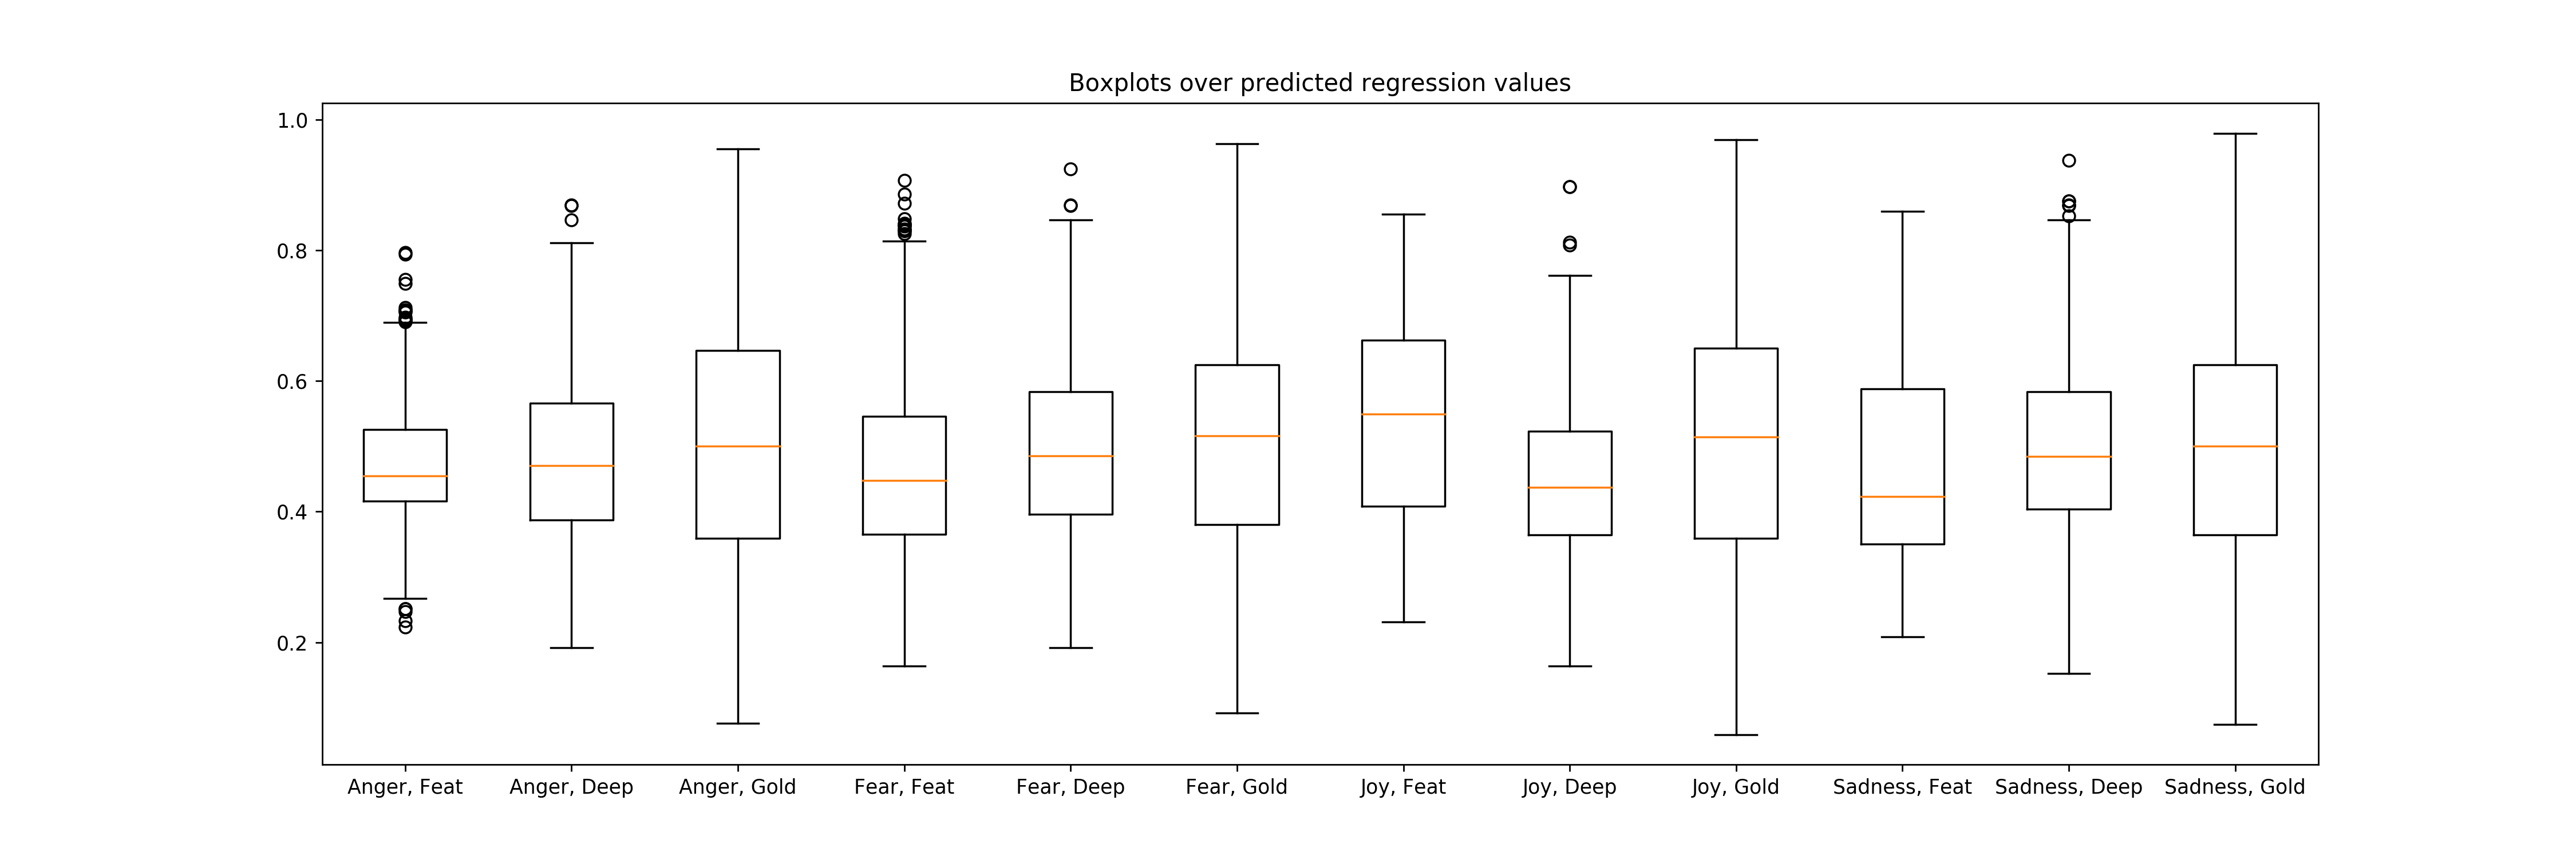
\includegraphics[width=\textwidth]{pictures/boxplotmix.png}
        \caption{The range of the two models predictions on regression data}
        \label{fig:boxplot}
\end{figure}
From figure \ref{fig:boxplot}, it is evident that none of the two models match the range of the gold scores. In general, both models suffer in the edgecases, where the scores are high ($>$ 0.8) and where they are low ($<$ 0.2). There are two instances where the difference between the two approaches is apparent, this being the scores with anger and joy tweets. The most favourable range in the joy case is reached with the feature based model, and this is reflected in the scores seen in section \ref{sec:featscores} and \ref{sec:deepscores} (Pearson score of 0.429 for the feature based model, 0.184 for the deep learning model). This difference can be explained by looking at the way the model generates predictions. Since the feature based model generates a new submodel for each feeling, the specific  submodel specializes in predicting one specific emotion, not considering a general, objective understanding of the words and their emotionality.\\
This is attempted by the deep learning model, but what happens with the data augmentation and by combining all tweets into one large pool is an implicit stripping of the emotionality of the tweets. An analogy would be to consider each tweet as a vector, with the regression emotion being the direction and the regression value being the magnitude of this vector. By combining all tweets in to one great pool (and by having tweets appear under different feelings and with different regression values) and by attempting to solve task 1 with one model and one set of weights/parameters, the direction of the "tweet vector" is stripped, and only magnitude is considered. This analogy can help understand why and how the model will predict when the tweet has four different gold labels in four different emotions (as seen in section \ref{sec:regscoredeep}).\\
\\
For a low level comparison, two exemplary tweets with multiple regression labels are used to represent the difference between the models.
\begin{table}[H]
\begin{tabular}{c|c|c|c|}
\parbox[t]{6cm}{\textit{'we need to do something. something must be done!!!!!' your anxiety is amusing. nothing will be done. despair.}} & Gold score & Feat prediction & Deep prediction \\ \hline
Anger & 0.517 & 0.477 & 0.761\\ \hline
Fear & 0.800 & 0.812 & 0.761\\ \hline
Joy & 0.197 & 0.376 & 0.761\\ \hline
Sadness & 0.707 & 0.574 & 0.761
\end{tabular}
\\[2ex]
\begin{tabular}{c|c|c|c|}
\parbox[t]{6cm}{\textit{What is this miserable ass weather all about \includegraphics[scale=0.015]{pictures/loudly_crying_face_emoji.png} dark and gloomy \#depressing \#weekoff \#wheresthesun}} & Gold score & Feat prediction & Deep prediction \\ \hline
Anger & 0.773 & 0.46 & 0.777\\ \hline
Fear & 0.6 & 0.526 & 0.777 \\ \hline
Joy & - & - & - \\ \hline
Sadness & 0.955 & 0.739 & 0.777
\end{tabular}
\caption{Tweet with scores for gold, feature based and deep learning scores}
\label{tab:predcomp}
\end{table}
In table \ref{tab:predcomp} it is apparent that the feature based predictions can vary drastically from the the deep learning predictions, and sometimes in a positive way, as the general scoring of joy tweets indicates.\\
One thing to note with the error analysis presented is that these are a general subsample of a larger whole. There is a larger amount of the tweets which are unique or might share two emotion regression values, and for these, the deep learning model is superior to the feature based model. The fact that joy is such an outlier in comparison to the other emotions drags the deep learning model down significantly.   

\subsection{Feature based}
\subsubsection{Custom features and effects}
All the custom features introduced in \ref{sec:customfeat} are boolean in nature; they consist of a check for whether or not a condition holds. This is a result of the relative ease with which one can engineer such features. The only value that would need any tweaking would be the ratio with which the spelling feature would be set, and this was deduced on a purely experimental basis. To a certain degree the positive and negative emojis are also a question of selecting and agreeing on which emojis are inherently positive and negative, but these were kept short and rather general.

\subsubsection{Difference between bag-of-words and deep learning}
The two models are built on two differing views when it comes to understanding text. The bag-of-words approach reduces the text to a large heap of words. By doing so, all interplay within the ordering of the words and syntax is removed. With the deep learning approach, a concept of keeping the syntax and the "human" way of reading is text is kept. This is because of the way the GRU keeps a state updated depending on the word being read but also the previous state. Instead of trying to infer meaning by using intricately designed features on a occurrences alone, the deep learning treats a tweet as a sequence, with possibly relevant structures intact. \\
Although neural networks and deep learning methods are prevalent in the literature, one should not disregard custom features as a addition. This is clear when looking at the results from last years SemEval task \cite{wassa2017}.

\subsection{Deep learning}
\subsubsection{What should the model do and how should it do it?}
A choice was taken early in the process that the model should be as general as possible and take as much data with differing truth labels as possible. The model, as of now, takes the truth labels from task 1 and task 5. These two tasks were chosen because of their relatedness with regards to emotion inference from tweets, but difference in that they require regression and classification. The difference between task 1 and task 2 seem trivial, in that a 0-to-1 regressional value can be mapped to an ordinal classification with relative ease, but the mapping from 0-to-1 regressional value to 11 binary flags, indicating emotions felt or not, seemed to require a more elaborate structure and loss function balancing.\\
\\
One thing of note is the way the data from task 1 is used in the final model. The regressional values are indirectly interpreted more as the outputs of a model trying to solve task 3 (\textit{Given a tweet, determine the intensity of sentiment or valence (V) that best represents the mental state of the tweeter—a real-valued score between 0 (most negative) and 1 (most positive)}) since emotionality is stripped implicitly. This is not the objective this data has been annotated towards, this has been annotated with regards to 4 specific emotions, but since the emotion of these scores are not directly evident from the output of the model, the scores can be considered to be more directly dependent of the classification label outputs. This is not necessarily the most meaningful way of guessing emotion intensities but it makes sense within the context of the task the model solves.

\subsubsection{Model iterations} \label{sec:iter}
The first baby steps towards a multitask learning model was reached by solving the regression task first and having a secondary output which consisted of a 4 dimensional vector with sigmoid activation and a single output using a softmax layer which indicated which regression emotion was felt. This classification was easily implemented since the truth labels were readily available because of the regression task needing 4 different emotion groupings. This way of classifying tweets could be reintroduced as to avoid the ambiguity of the regression value output in the models current state.\\
The first iteration of the model that attempted to solve task 5 had a different output layer/loss function constellation with regards to the classification of the tweets. It had a single, 11 dimensional output vector which corresponded to the full classification label list. This model would have a high degree of skew and very low range, and this was the product of having a single layer with a limited amount of weights to be tweaked on. Since an average label list had a high amount of zeros (as shown in table \ref{tab:skew}) the weighting for the classification output layer would have a tendency to guess zeros and since there was not enough parameters to be tweaked, the results would end up looking the same for all tweets.\\
The last, and current model iteration has 11, one-dimensional output vectors, one for each classification label. The ability to tweak weights on a per-label basis ended up in the most meaningful predictions from the overall model architecture.

\subsubsection{Loss functions; how to model the classification} \label{sec:lossdiscussion}
As can be seen in table \ref{tab:skew}, flags are skewed towards certain emotions. This uneven distribution might have something to do with the ease of labelling a tweet with the emotions. Since the train, dev and test data for the task has been manually labelled, certain "human" effects might be felt and can be backpropagated through to the models built on the data. For instance, it might be very easy to infer anger in a tweet; an exclamation mark, a curse word or something similar might be used to infer the feeling, but how can you infer surprise? Or trust? Furthermore, 274 of the tweets had no feeling flags set, which was to be understood as a "neutral" feeling.\\
\begin{table}[H]
\scalebox{0.8}{\begin{tabular}{c|c|c|c|c|c|c|c|c|c|c|c|}
& \text{Anger} & \text{Anticipation} & \text{Disgust} & \text{Fear} & \text{Joy} & \text{Love} & \text{Optimism} & \text{Pessimism} & \text{Sadness} & \text{Surprise} & \text{Trust} \\ \hline
\text{\# of flags set} & 2605 & 990 & 2666 & 1269 & 2499 & 699 & 2007 & 812 & 2076 & 365 & 352 \\
\text{\% of tweets} & 38\% & 14\% & 39\% & 19\% & 37\% & 10\% & 29\% & 12\% & 30\% & 5\% & 5\%
\end{tabular}}
\caption{The actual flags set and percentage of the full classification dataset}
\label{tab:skew}
\end{table}
The metric, equation (\ref{eq:accuracy}), used can be problematic since it completely disregards tweets with zero flags set, which otherwise could present a nice and diverse understanding of feelings and their interplay on how people will write their tweets. The secondary official metrics are also problematic in that they also disregard "neutral" tweets. To mitigate this, the evaluation script used for local evaluation included a twelfth dimension which was only set if all the others were not. This allowed for a more nuanced picture in the edge case where all of the flags were not set.

\subsubsection{Lexicons and features}
Since the model was built with simplicity in mind, a choice was made early on that the model should use as little data as possible that was not included in the train, development and test sets. Since the weights were to be pretrained, those represented extra data, but otherwise the models takes as input only the data given in the task. That said, there was many more data sources that could be considered.\\
Emoji lexicons was one of them. Emojis are prevalent on twitter and they convey a lot of meaning in a difficult-to-map manner, meaning they sometimes might be used in an ironic or otherwise non-fitting situation. Take, for example:\\
\begin{center}
\textit{Can I just sulk in peace} \includegraphics[scale=0.015]{pictures/tears_of_joy_emoji.png}
\end{center}
This tweet has a gold value of 0.688 in sadness, but looking at the smiley alone would tell a very different story than the feeling being conveyed by the whole tweet. This sort of intricate, feature-like nature of emojis could warrant a seperate usage of lexicons so as to augment the word embeddings, only for emojis. This trend is apparent in \cite{wassa2017} where it is specified that 6 teams used emoji lexicons or an embedding used solely for emojis.\\
\\
Furthermore, sentiment lexicons is a resource that 9 out of the top 10 from the WASSA-2017 Shared Task used. These were used in the same general way; a lookup in the lexicons is done for each word in the tweet, the number of occurences in each lexicon is then counted up. A supplied intensity score was sometimes used to further augment the summation, as shown in \cite{seernet}. These were then used as more traditional linguistic features and fed to the models.\\
A model that used very few external sources of data was the model presented in \cite{hpcc}. The overall architecture looked very similar to the one presented in this report, and this model received an average Pearson score of 0.671 and a 7th place in the task.